% Options for packages loaded elsewhere
\PassOptionsToPackage{unicode}{hyperref}
\PassOptionsToPackage{hyphens}{url}
%
\documentclass[
]{article}
\usepackage{amsmath,amssymb}
\usepackage{iftex}
\ifPDFTeX
  \usepackage[T1]{fontenc}
  \usepackage[utf8]{inputenc}
  \usepackage{textcomp} % provide euro and other symbols
\else % if luatex or xetex
  \usepackage{unicode-math} % this also loads fontspec
  \defaultfontfeatures{Scale=MatchLowercase}
  \defaultfontfeatures[\rmfamily]{Ligatures=TeX,Scale=1}
\fi
\usepackage{lmodern}
\ifPDFTeX\else
  % xetex/luatex font selection
\fi
% Use upquote if available, for straight quotes in verbatim environments
\IfFileExists{upquote.sty}{\usepackage{upquote}}{}
\IfFileExists{microtype.sty}{% use microtype if available
  \usepackage[]{microtype}
  \UseMicrotypeSet[protrusion]{basicmath} % disable protrusion for tt fonts
}{}
\makeatletter
\@ifundefined{KOMAClassName}{% if non-KOMA class
  \IfFileExists{parskip.sty}{%
    \usepackage{parskip}
  }{% else
    \setlength{\parindent}{0pt}
    \setlength{\parskip}{6pt plus 2pt minus 1pt}}
}{% if KOMA class
  \KOMAoptions{parskip=half}}
\makeatother
\usepackage{xcolor}
\usepackage[margin=1in]{geometry}
\usepackage{longtable,booktabs,array}
\usepackage{calc} % for calculating minipage widths
% Correct order of tables after \paragraph or \subparagraph
\usepackage{etoolbox}
\makeatletter
\patchcmd\longtable{\par}{\if@noskipsec\mbox{}\fi\par}{}{}
\makeatother
% Allow footnotes in longtable head/foot
\IfFileExists{footnotehyper.sty}{\usepackage{footnotehyper}}{\usepackage{footnote}}
\makesavenoteenv{longtable}
\usepackage{graphicx}
\makeatletter
\def\maxwidth{\ifdim\Gin@nat@width>\linewidth\linewidth\else\Gin@nat@width\fi}
\def\maxheight{\ifdim\Gin@nat@height>\textheight\textheight\else\Gin@nat@height\fi}
\makeatother
% Scale images if necessary, so that they will not overflow the page
% margins by default, and it is still possible to overwrite the defaults
% using explicit options in \includegraphics[width, height, ...]{}
\setkeys{Gin}{width=\maxwidth,height=\maxheight,keepaspectratio}
% Set default figure placement to htbp
\makeatletter
\def\fps@figure{htbp}
\makeatother
\setlength{\emergencystretch}{3em} % prevent overfull lines
\providecommand{\tightlist}{%
  \setlength{\itemsep}{0pt}\setlength{\parskip}{0pt}}
\setcounter{secnumdepth}{5}
\usepackage{subfig}
\usepackage{float}
\ifLuaTeX
  \usepackage{selnolig}  % disable illegal ligatures
\fi
\usepackage{bookmark}
\IfFileExists{xurl.sty}{\usepackage{xurl}}{} % add URL line breaks if available
\urlstyle{same}
\hypersetup{
  pdftitle={EDA},
  pdfauthor={Yufei Liu},
  hidelinks,
  pdfcreator={LaTeX via pandoc}}

\title{EDA\thanks{Code and data are available at: \url{https://github.com/Florence-Liu/Stellar-Flare}}}
\author{Yufei Liu}
\date{2025-02-09}

\begin{document}
\maketitle

\section{Data summary}\label{data-summary}

In this project, we are interested in detecting stellar flares using different methods and compare the model performance for three stars using TESS light curve data for TIC 0131799991, TIC 129646813, and TIC 031381302. We mainly focused on two variables from the dataset, time and PDCSAF Flux, which refers to the corrected flux after summing the calibrated pixels within the TESS optimal photometric aperture. The original dataset, although, includes missing values for both flux and time, which could be a problem when we modeling the data.

For the following exploratory data analysis, I will use data for TIC 013799991 as an example, and will expand the implements to other two stars.

It is noticeable for TIC 013799991 that it actually has a missing period between time index 1529 to 1535 as shown in Table \ref{tab:summary}, which may be the result of instrumental errors. For the missing values in flux, as shown in Figure \ref{fig:ts-2}, the heatmap shows that only the very first a few observations are missing (observation in light blue). In this case, since the time in the data refers to the Barycentric Julian Date, instead of converting it to a \texttt{ymd} variable, I kept the original numeric number since I found it is unnecessary to convert and may introduce extra errors in the process. So the heatmap did not show the missing period in time.

\begin{figure}[H]

{\centering \subfloat[Time Series Plot\label{fig:ts-1}]{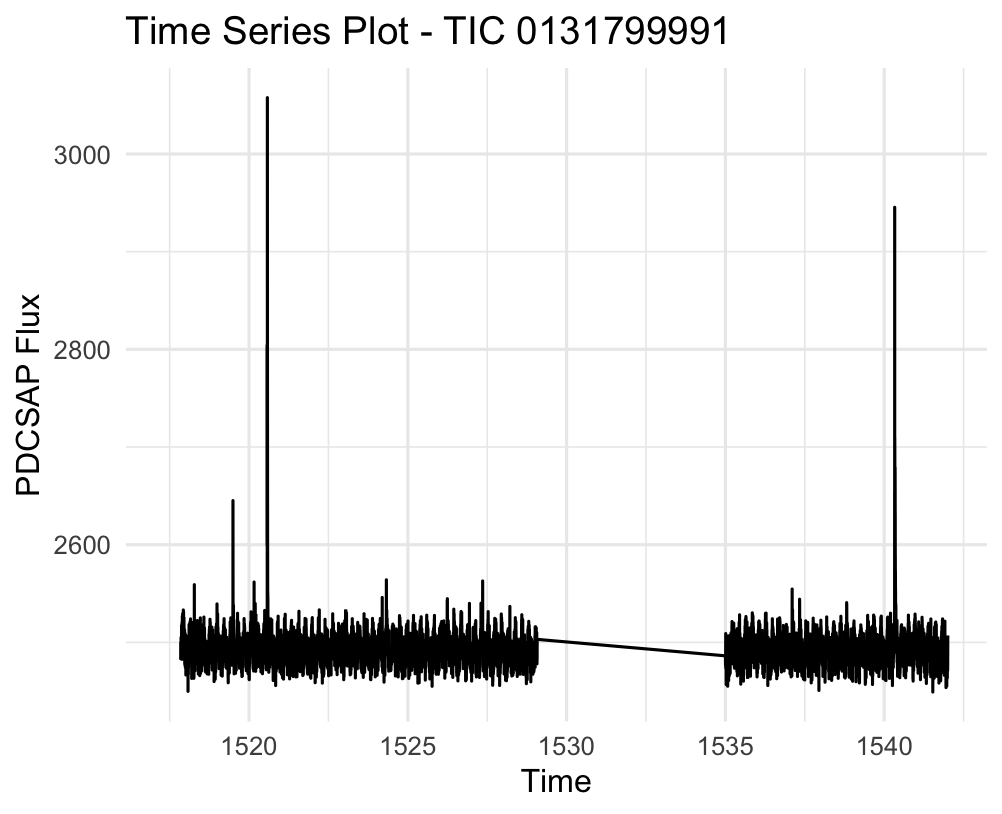
\includegraphics[width=0.5\linewidth]{Figure/ts_plot_before_013} }\subfloat[Heatmap\label{fig:ts-2}]{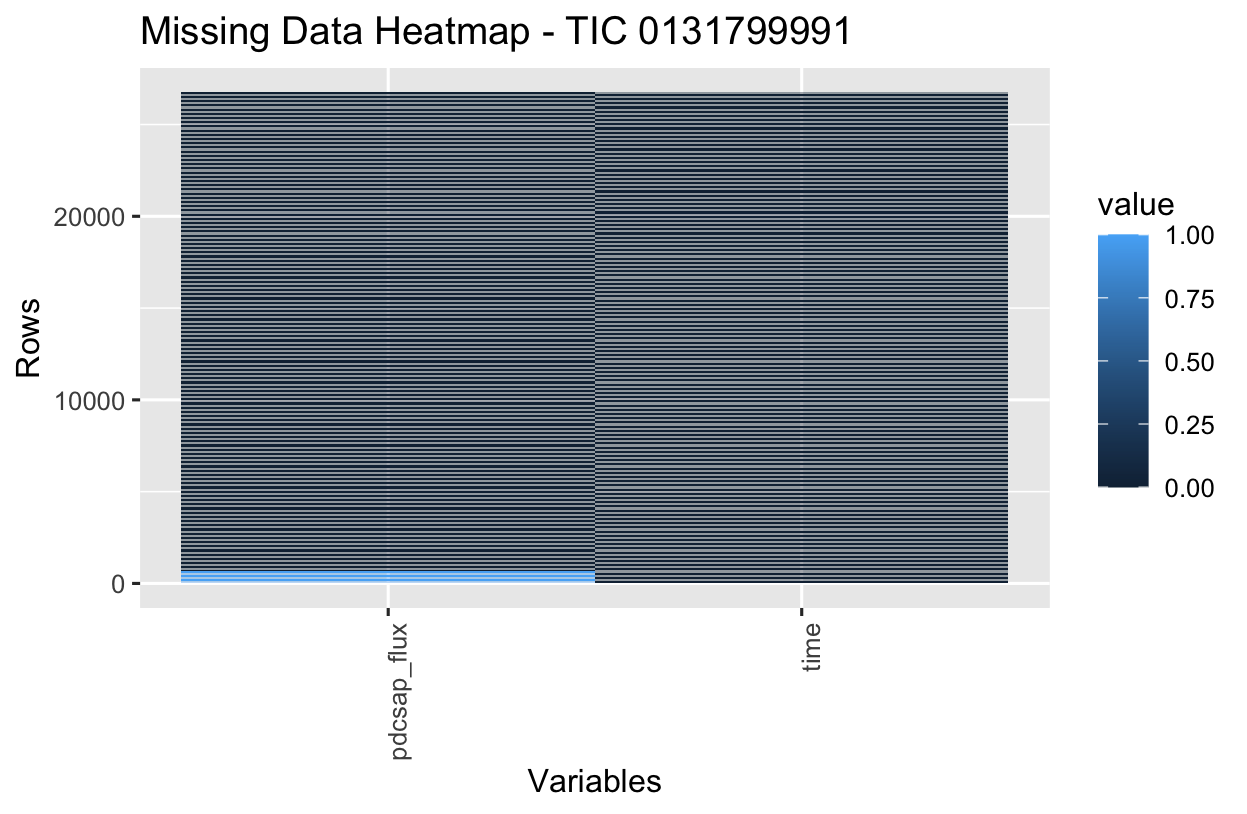
\includegraphics[width=0.5\linewidth]{Figure/heatmap_013} }

}

\caption{Visualization of Time Series TIC 0131799991}\label{fig:ts}
\end{figure}

\begin{longtable}[]{@{}lrr@{}}
\caption{\label{tab:summary} Part of data with missing period}\tabularnewline
\toprule\noalign{}
Index & Time & PDCSAF Flux \\
\midrule\noalign{}
\endfirsthead
\toprule\noalign{}
Index & Time & PDCSAF Flux \\
\midrule\noalign{}
\endhead
\bottomrule\noalign{}
\endlastfoot
8343 & 1529.065 & 2484.593 \\
8344 & 1529.067 & 2478.021 \\
8345 & 1529.068 & 2503.103 \\
8346 & 1535.001 & 2486.231 \\
8347 & 1535.003 & 2476.867 \\
8348 & 1535.004 & 2486.383 \\
8349 & 1535.006 & 2487.144 \\
8350 & 1535.007 & 2479.111 \\
8351 & 1535.008 & 2488.168 \\
\end{longtable}

Since it is a time series data, I conducted the time series analysis to check some features of the dataset, including the ACF, PACF, and seasonal trend decomposition.

Figure \ref{fig:acf} shows the autocorrelation plots for the star, with different maximum lags. Figure \ref{fig:acf-1} shows autocorrelation for first 50 lags. We could see that the behaviour for the ACF shows a damped exponential dying down with oscillation, and in Figure \ref{fig:acf-2}, when I extended the ACF plot to 500 lags, we could see that there existing repeating peaks at around 150 after scaling, indicating the original time series is non-stationary. So I tried to take the first difference of the time series and got the new ACF as shown in \ref{fig:acf-3}, it looks like there are 5 spikes in the plot, indicating highly correlated lags.

\begin{figure}[H]

{\centering \subfloat[50 lags\label{fig:acf-1}]{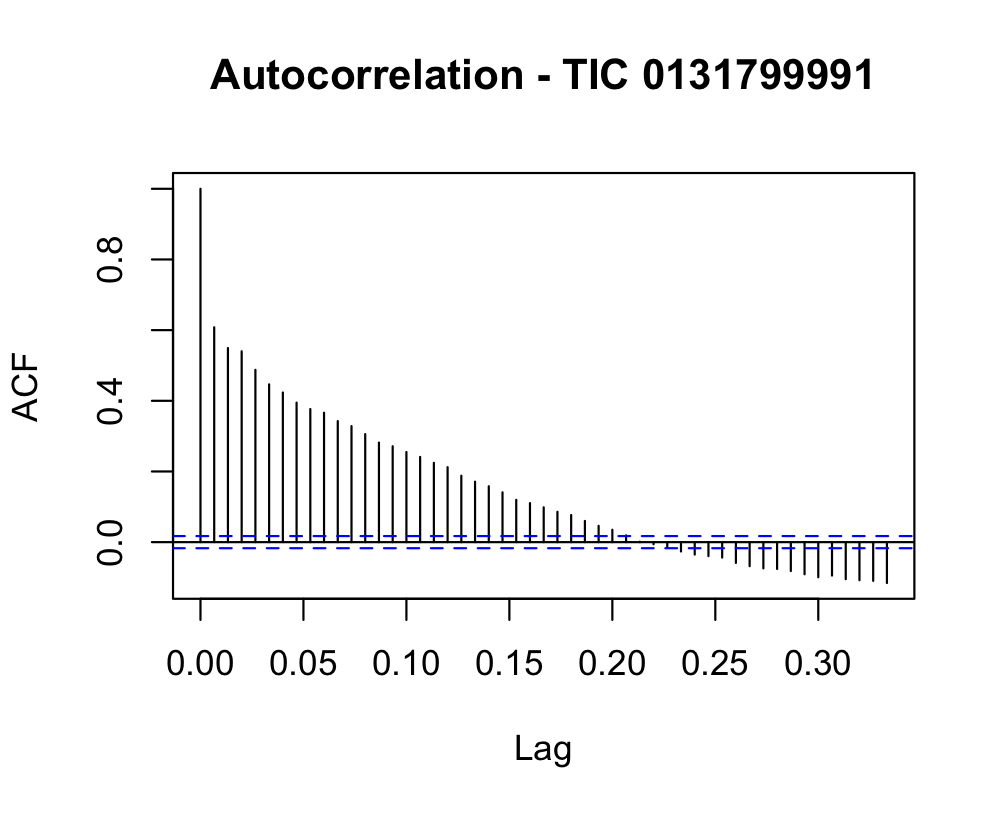
\includegraphics[width=0.35\linewidth]{Figure/ACF_013_max50} }\subfloat[First difference\label{fig:acf-2}]{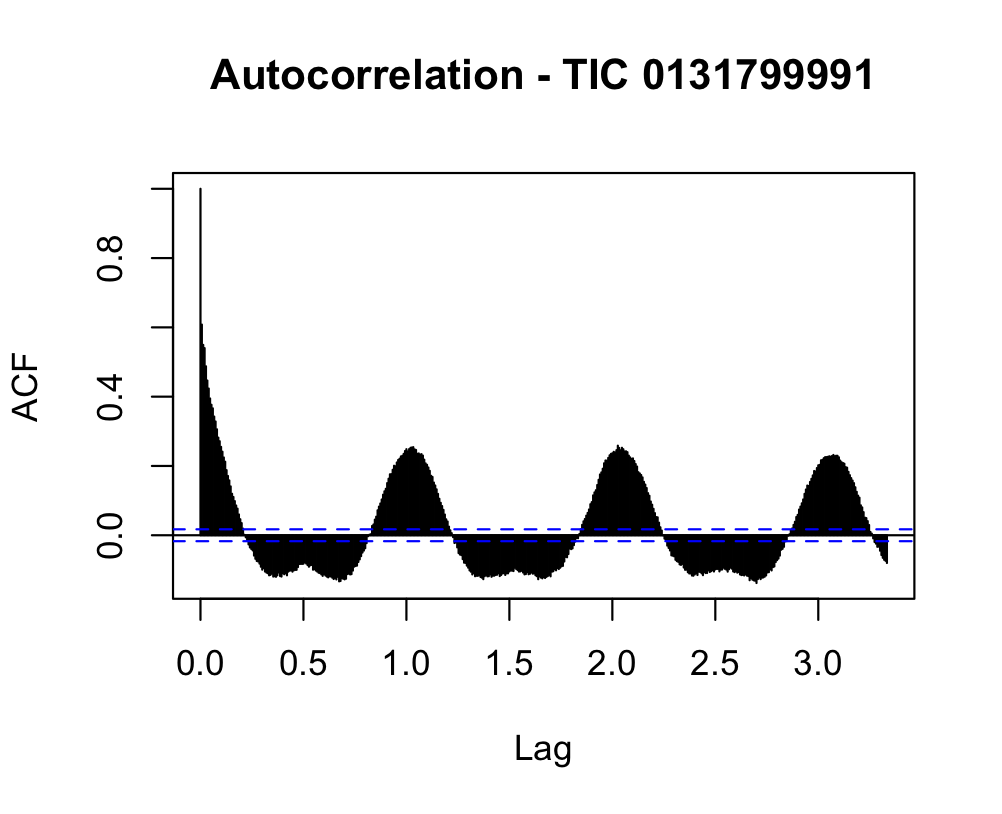
\includegraphics[width=0.35\linewidth]{Figure/ACF_013_max500} }\subfloat[500 lags\label{fig:acf-3}]{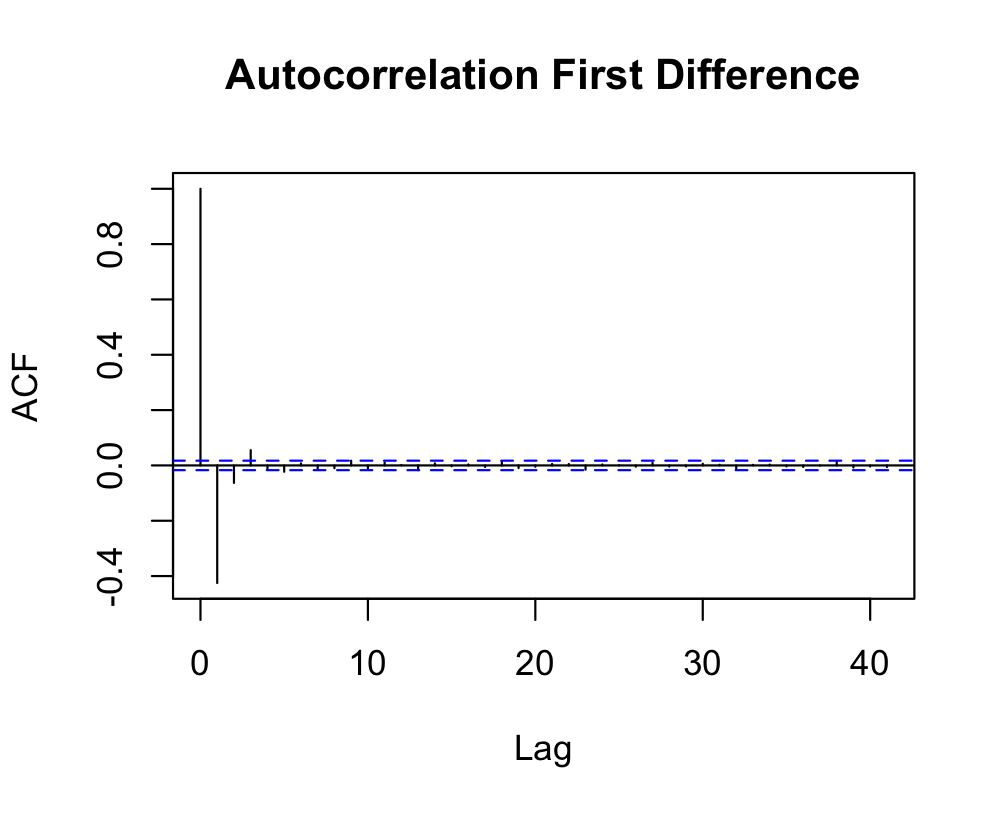
\includegraphics[width=0.35\linewidth]{Figure/first_difference_013} }

}

\caption{Autocorrelation Plots for Time Series TIC 0131799991}\label{fig:acf}
\end{figure}

Figure \ref{fig:stl-1} shows the Partial Autocorrelation plot for the original time series, we could see there are approximately 8 spikes, suggesting a AR(8) model may be useful. Combined with the ACF plots, an ARIMA model (8, 0, 4) \(\times\) (1, 0, 0) may be useful. To better see the trend and seasonality, I used the Seasonal-Trend Decomposition using Loess. As shown in Figure \ref{fig:stl-2}, there seems to be no seasonality in this data since the seasonal plot spreads equally around 0. For the trend, we could clear see that there are several local peaks, indicating the existence of flares, but needs to be furthur investigated. The most possible flares could occur at index 13 and index 80.

\begin{figure}[H]

{\centering \subfloat[PACF\label{fig:stl-1}]{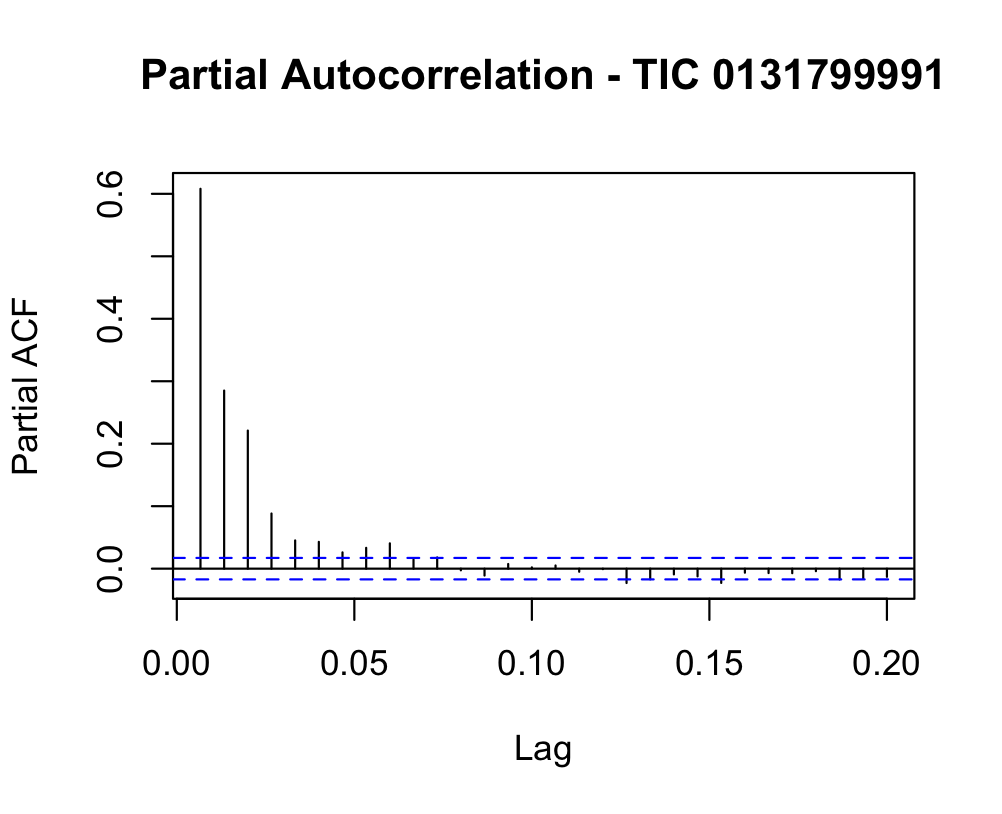
\includegraphics[width=0.5\linewidth]{Figure/PACF_013} }\subfloat[STL decompositioin\label{fig:stl-2}]{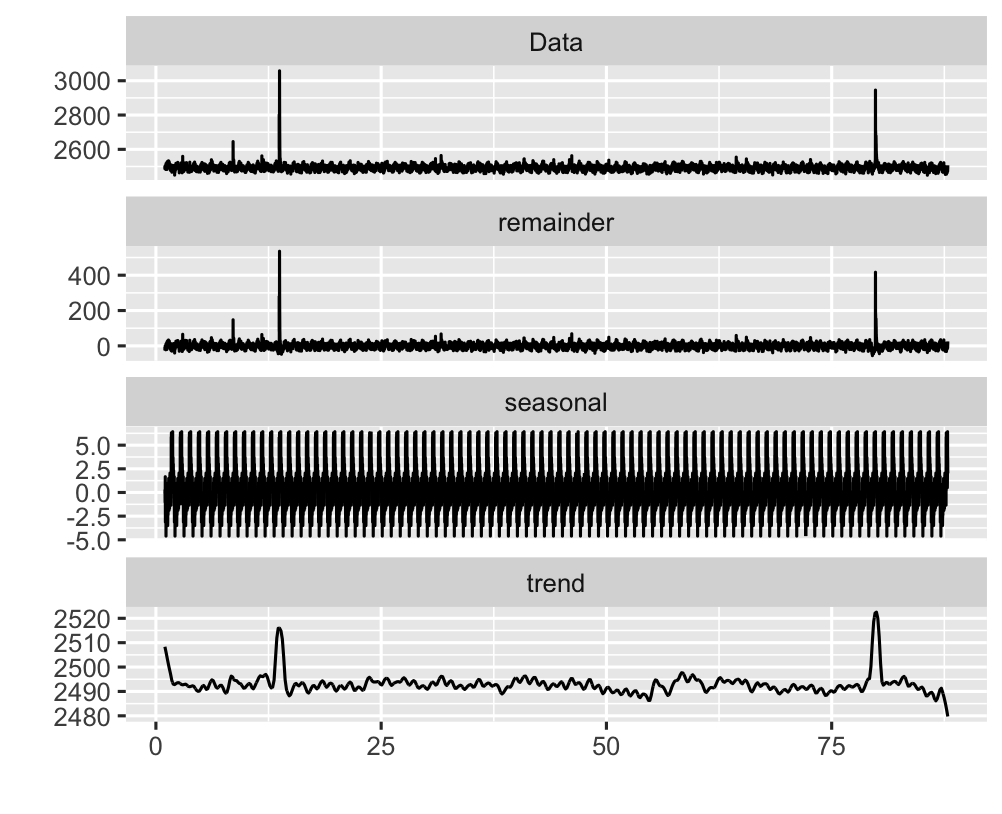
\includegraphics[width=0.5\linewidth]{Figure/decomposition_013} }

}

\caption{Result for Partial Autocorrelation and STL Decomposition}\label{fig:stl}
\end{figure}

\section{Handling missing data}\label{handling-missing-data}

Since I'm interested in comparing model performance for ARIMA Model, DBSCAN, and Gaussian Mixture Model, handling missing data is necessary for some these models (DBSCAN and ARIMA). In this case, I focused on the gap between 1529 and 1535, using several different methods First is to use the \texttt{imputeTS} package, which is a package used in \texttt{R} for univariate time series missing data imputations. I tried to use model-based imputations including ARIMA model and Exponentially Weighted Moving Average. I also tried rolling statistics approach. Another approach is to split the time series into pre-gap and post-gap datasets, using pre-gap data as training data to model and forecast the missing values.

Figure \ref{fig:imputes-1} shows that the result for ARIMA model using Kalman Smoothing and State-Space Representations. The yellow line fills the gap as well as the missing flux at the beginning. For Figure \ref{fig:imputes-2}, the exponentially weighted moving average gives a really bad result, which may because of the trend of original data and large gap.

Figure \ref{fig:rolling-1} shows the imputation result using rolling mean with window of 5, which means taking mean pf 5 closest observations to substitute the missing values. It is helpful since our missing data may be non-random, however, the choice of window size affects the result. Also, the our gap is relatively large, using mean of neighbours highly depends on the previous substitute result, so we could see that the effect is not that satisfying. Figure \ref{fig:rolling-2} shows the result for approach two, which I split the pre-gap data as training data to build an ARIMA model and forecast the missing values. In this case, I assumed that the behaviour during the missing period could be similar to the pre-gap period. The effect is not very good as for the time near the observed ones, the forecast could be useful, however, same problems happened as later forecast depend on the previous ones, making the forecast go to very similar values. This may due to the large forecast size I chose as for each time interval of 0.001.

\begin{figure}[H]

{\centering \subfloat[ARIMA\label{fig:imputes-1}]{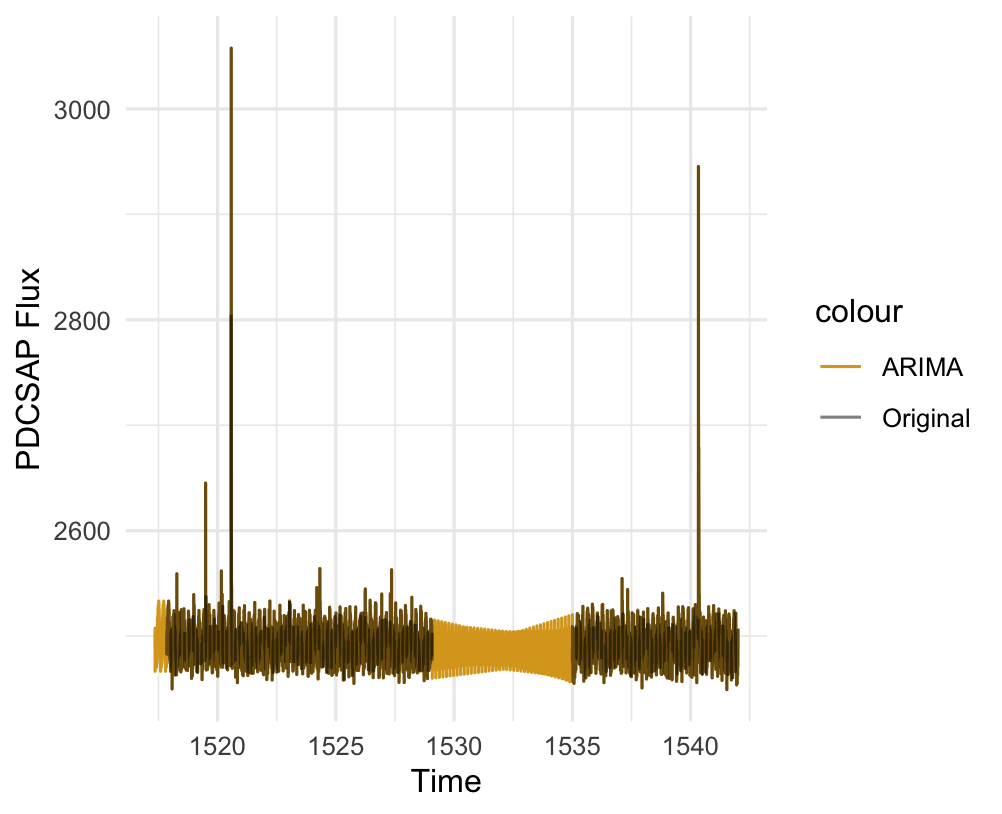
\includegraphics[width=0.5\linewidth]{Figure/ARIMA_imputeTS_013} }\subfloat[EWMA\label{fig:imputes-2}]{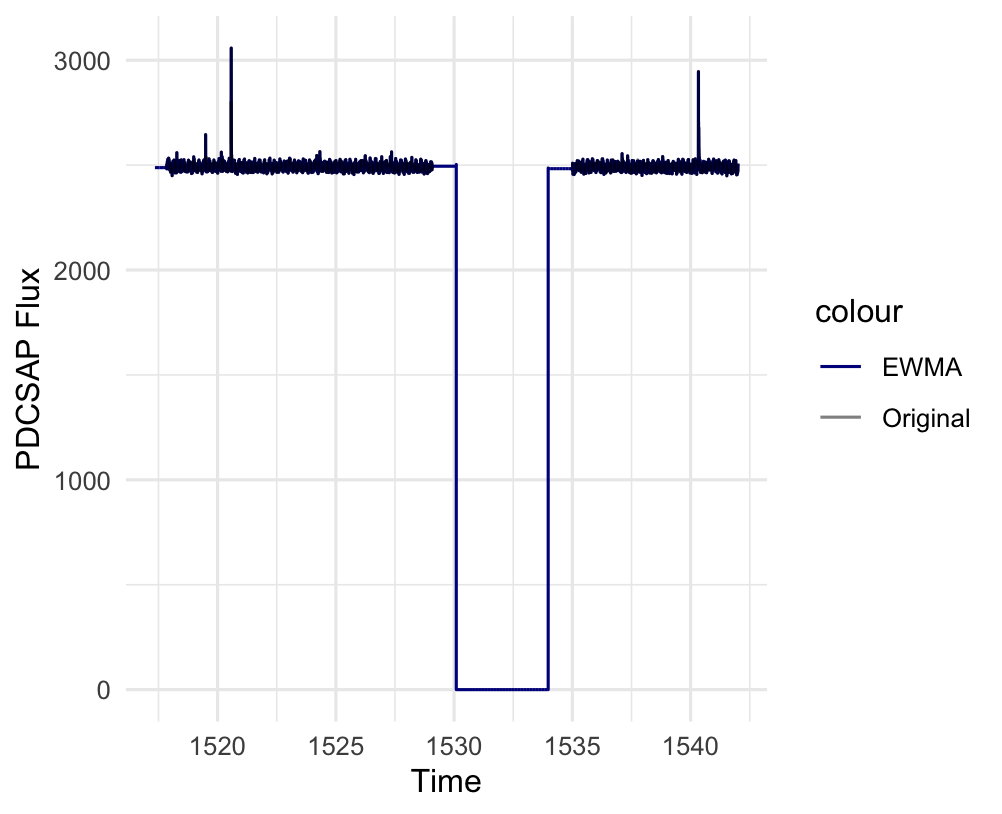
\includegraphics[width=0.5\linewidth]{Figure/EWMA_013} }

}

\caption{Result for Sample Imputation of Missing Data using ImputeTS package}\label{fig:imputes}
\end{figure}

\begin{figure}[H]

{\centering \subfloat[Rolling Mean\label{fig:rolling-1}]{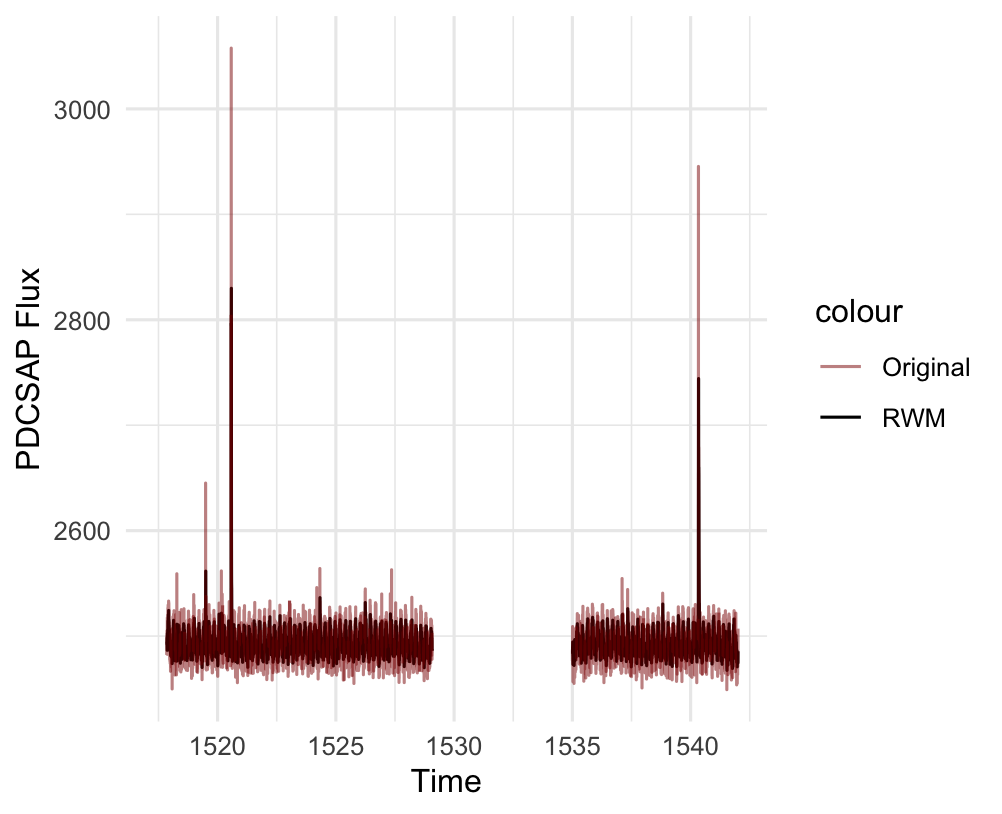
\includegraphics[width=0.5\linewidth]{Figure/Rolling_Mean_013} }\subfloat[Forecast\label{fig:rolling-2}]{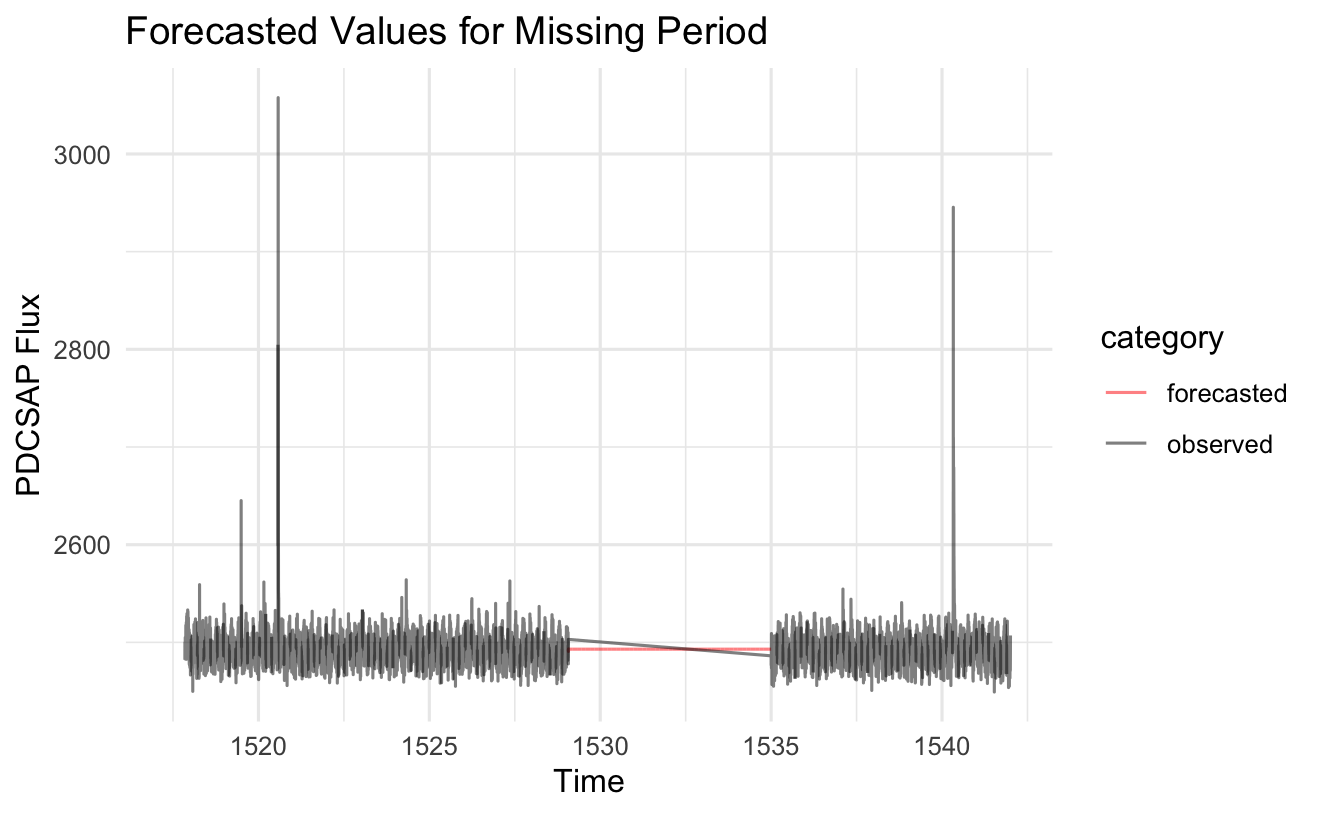
\includegraphics[width=0.5\linewidth]{Figure/Pre-gap_imputation_013} }

}

\caption{Result for Sample Imputation of Missing Data using Rolling Window Mean and Forecast}\label{fig:rolling}
\end{figure}

The final thought was to simply remove the missing values and consider model the time series separately, i.e.~pre-gap and post-gap. As shown in Figure \ref{fig:ts-2}, the missing values of flux, the variable we care about, have a very small proportion, which may not affect a lot on the model performance. In this case, we still assume the behaviour during the missing period is similar to that in the observed data.

\end{document}
